\section{Auswertung}
\label{sec:Auswertung}
Jegliche Fehlerrechnung wurde mit der python-Bibliothek uncertainties \cite{uncertainties} absolviert.
Trotz dessen sind die Formeln für die Unsicherheiten in den jeweiligen Abschnitten angegeben.
Allgemeine Rechnungen wurden mit der python-Bibliothek numpy \cite{numpy} automatisiert. 
Die Messdaten und Ausgleichskurven wurden mit Hilfe der python-Bibliothek matplotlib \cite{matplotlib} erstellt.\\
Die Spannung $U_0$ beträgt bei allen Durchführungen $\SI{6.4}{\volt}$.
\subsection{Bestimmung der Zeitkonstante mit dem Entladevorgang}
Die während der Durchführung gemessenen Werte für $U_\text{C}$ in Abhängigkeit von der Zeit sind in Tabelle \ref{tab:UCt} aufgeführt.
\begin{table}
    \centering
    \caption{Gemessene Kondensatorspannung $U_\text{C} \left (t \right )$}
    \label{tab:UCt}
    \begin{tabular}{S[table-format=1.1] S[table-format = 1.1]}
        \toprule
        {$ t \mathbin{/} \si{\milli\second}$} & {$U_\text{C} \mathbin{/} \si{\volt}$} \\
        \midrule
        0   & 6.2 \\
        0.1 & 5.3 \\
        0.2 & 4.7 \\
        0.3 & 4.1 \\
        0.4 & 3.5 \\
        0.5 & 2.9 \\
        0.6 & 2.5 \\
        0.7 & 1.9 \\
        0.8 & 1.5 \\
        0.9 & 1.1 \\
        1   & 0.7 \\
        1.1 & 0.5 \\
        1.2 & 0.1 \\
        \bottomrule        
    \end{tabular}
\end{table}
\begin{figure}
        \centering
        \caption{Verlauf der Spannung bei einem Entladevorgang}
        \label{fig:discharge}
        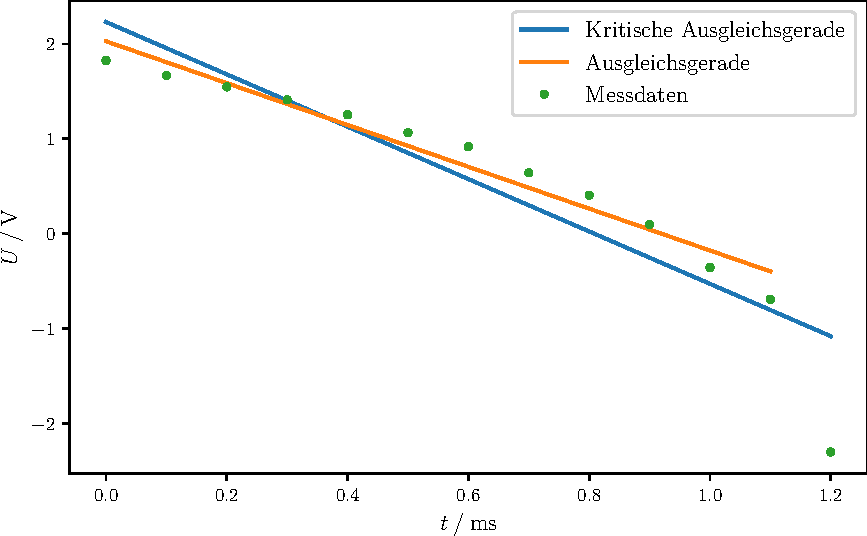
\includegraphics{build/uct.pdf}
\end{figure}
Bei dem Spannungsverlauf in Abblidung \ref{fig:discharge} ist zunächst anzumerken, dass dort zwei Ausgleichsgeraden angelegt wurden. 
Dies liegt der Ursache zu Grunde, dass der letzte Punkt der Messreihe eine sehr starke Abweichung zeigt.
Die gesamte Ausgleichsgerade beschreibt die komplette Messreihe, wobei der letzte Messwert bei der kritischen Ausgleichsgerade ausgelassen wurde.
Im Folgenden werden die Rechungen mit den Parametern der kritischen Ausgleichsgeraden durchgeführt.
Für die Bestimmung der Zeitkonstanten $RC$ wird die Gleichung \eqref{eqn:Charge} verwendet.
Jedoch wird die Ladung $Q$ durch die Spannung $U_\text{C}$ ersetzt.
Umgestellt und logarithmiert ergibt sich 
\begin{equation}
    \ln \left( \frac{U_\text{C}}{U_0} \right ) =  - \frac{t}{RC} \; \text{.} 
\end{equation} 
Die Ausgleichsgerade hat die Form $ \ln \left( \sfrac{U_\text{C}}{U_0} \right ) = at + b$, wobei $a = - \sfrac{1}{RC}$ gilt.
Die Parameter haben die Werte 
\begin{align*}
    a &= \SI{-0.3447(229)}{\per\milli\second} \\
    b &= \num{0.3169(149)} \; \text{.}
\end{align*}
Der Wert für $a$ in $RC = - \sfrac{1}{a}$ eingesetzt ergibt
\begin{equation*}
   RC = \SI{2.90(19)}{\milli\second} \; \text{.}
\end{equation*}
Nach jeder Ausgleichsrechnung erhält man die Zeitkonstante direkt durch einen Paremeter der Ausgleichsfunktion.
Jedoch bildet dieser Teil der Auswertung eine Ausnahme, denn hier wird die Zeitkonstante mit $RC = - \sfrac{1}{a}$ errechnet, so dass hier die Formel der Gaußschen
Fehlerfortpflanzung angewendet werden muss.
Somit ergibt sich der Fehler der Zeitkonstante zu 
\begin{equation}
    \symup{\Delta} RC = \abs*{\frac{1}{a}} \, \symup{\Delta} a \; \text{.}
\end{equation}
\subsection{Frequenzabhängige Spannunsgmessung}
Die Messwerte für die Kondensatorspannung $U_\text{C}$ in Abhängigkeit von der Frequenz $\omega$ sind in Tabelle \ref{tab:ucw} aufgelistet.
\begin{table}
    \centering
    \caption{Gemessene Kondensatorspannung $U_\text{C} \left( \omega \right)$}
    \label{tab:ucw}
    \begin{tabular} {S[table-format = 4.0] S[table-format = 1.4]}
        \toprule
        {$\omega \mathbin{/} \si{\hertz}$} & {$U_\text{C} \mathbin{/} \si{\volt}$}\\
        \midrule
        10    & 6.4    \\
        20    & 6.4    \\
        40    & 6.2    \\
        60    & 6.0    \\
        80    & 5.6    \\
        100   & 5.4    \\
        200   & 3.6    \\
        400   & 2.0    \\
        600   & 1.4    \\
        800   & 1.05   \\
        1000  & 0.85   \\
        2000  & 0.44   \\
        4000  & 0.2    \\
        6000  & 0.014  \\
        8000  & 0.0105 \\
        10000 & 0.0085 \\
        \bottomrule
    \end{tabular}
\end{table}
Um die nichtlineare Ausgleichskurve anlegen zu können, wird zunächst die Funktion der Amplitude benötigt, welche in Gleichung \eqref{eqn:ampli} aufgeführt ist. 
Fortlaufend wird zur Vereinfachung $R^2C^2$ zu $\tau^2$ umdefiniert.
Die Frequenz $\omega$ wird zur Klarifizierung in $x$ umbenannt.
Somit nimmt die Funktion der Ausgleichskurve die Gestalt
\begin{equation}
    f(x) = \frac{U_\text{C}}{U_0} \left( x \right) = \frac{1}{\sqrt{1 + x^2 \tau^2}}
\end{equation}
an.
Mittels der Ausgleichsrechnung in python ergibt sich $\tau$ zu 
\begin{equation*}
    \tau = \SI{-7.1653(1441)}{\milli\second} \; \text{.}
\end{equation*}
Somit ergibt sich die Zeitkonstante $RC$ zu   
\begin{equation}
    RC =  \SI{7.1653(1441)}{\milli\second} \; \text{.}
\end{equation}
Die Messdaten samt Fit sind in Abbildung \ref{fig:ucw} visualisiert.
\begin{figure}
    \centering
    \caption{Kondensatorspannung $U_\text{C} \left( \omega \right)$}
    \label{fig:ucw}
    \includegraphics{build/ucw.pdf}
\end{figure}
\subsection{Bestimmung der Zeitkonstante mittels frequenzabhängiger Phasenverschiebung}
Die Messwerte für die Frequenz $\omega$, der Zeitabstände der Nulldurchgänge $a$ und der Schwingungsdauern $b$ sind in Tabelle \ref{tab:ab} aufgetragen.
Zusätzlich beinhaltet diese Tabelle die aus den Messdaten berechneten Phasenverschiebungen, welche sich mittels  Gleichung \eqref{eqn:phiab} berechnen lassen.
\begin{table}
    \centering
    \caption{Gemessene Frequenz, Zeitabstände der Nulldurchgänge $a \left ( \omega \right )$,  Schwingungsdauern $b \left ( \omega \right )$ und berechnete
    Phasenverschiebung $\varphi \left ( \omega \right )$}
    \label{tab:ab}
    \begin{tabular}{S[table-format = 4.0] S[table-format = 1.3] S[table-format = 3.3] S[table-format = 1.2]}
        \toprule
        {$\omega \mathbin{/} \si{\hertz}$} & {
        $a \mathbin{/} \si{\milli\second}$} & 
        {$b \mathbin{/} \si{\milli\second}$} &
        {$\varphi \mathbin{/} \si{\radian}$} 
        \\
        \midrule
        10    & 1.2   & 110   & 0.07 \\
        20    & 1.5   & 55    & 0.17 \\
        40    & 1.7   & 25    & 0.42 \\
        60    & 1.15  & 16.6  & 0.44 \\
        80    & 1.1   & 12.6  & 0.55 \\
        100   & 1.08  & 10    & 0.68 \\
        200   & 0.8   & 5     & 1.01 \\
        400   & 0.52  & 2.5   & 1.31 \\
        600   & 0.36  & 1.7   & 1.33 \\
        800   & 0.28  & 1.24  & 1.42 \\
        1000  & 0.23  & 1     & 1.45 \\
        2000  & 0.12  & 0.49  & 1.54 \\
        4000  & 0.06  & 0.25  & 1.51 \\
        6000  & 0.04  & 0.168 & 1.5  \\
        8000  & 0.031 & 0.128 & 1.52 \\
        10000 & 0.024 & 0.1   & 1.51 \\
        \bottomrule
    \end{tabular}
\end{table}
Um die Zeitkonstante mit Hilfe der Phasenverschiebung graphisch zu bestimmen, wird die Gleichung \eqref{eqn:ficken} benötigt.
Erneut wird die Zeitkonstante $RC$ zu $\tau$ umdefiniert und die Frequenz $\omega$ in $x$ unbenannt.
Somit erhält die Ausgleichskurve die Darstellung 
\begin{equation}
    f \left( x \right) = \varphi \left ( x \right ) = \arctan \left( - x \tau \right) \;\text{.}
\end{equation}
\begin{figure}
    \centering
    \caption{Phasenverschiebung $\varphi \left ( \omega \right )$}
    \label{fig:phiw}
    \includegraphics{build/phasefreq.pdf}
\end{figure}
\noindent Durch Ausgleichsrechnung in python ergibt sich der Parameter $\tau$ zu 
\begin{equation*}
    \tau = \SI{-8.2744(3239)}{\milli\second} \; \text{.}
\end{equation*}
Somit wird der Wert der Zeitkonstanten $RC$ mit der Methode der Phasenverschiebung zu
\begin{equation*}
    RC =     \tau = \SI{8.2744(3239)}{\milli\second}
\end{equation*}
bestimmt. Das Verhältnis $\sfrac{A \left ( \omega \right )}{U_0}$ in Abhängigkeit von der Phase $\varphi$ ist in einem Polarplot in Abbildung \ref{fig:polar} dargestellt.
\begin{figure}
    \centering
    \caption{Polarplot von der Amiplitude $A \left( \varphi \right)$}
    \label{fig:polar}
    \includegraphics{build/polar.pdf}
\end{figure}
\newpage
\subsection{Der RC-Kreis als Integrator}
Der RC-Kreis kann unter der Voraussetzung 
\begin{equation}
     \omega >> \frac{1}{RC} 
\end{equation}
als Integrator angesehen  werden.
Bei der Aufnahme der folgenden Bilder wurde die Bedingung mit einer hohen Frequenz erfüllt.
Somit enstanden die Impressionen der Rechteck-, Sinus- und Dreiecksspannung.
Beispielsweise wird an der Abbildung \ref{fig:sin} sehr schön deutlich, dass der RC-Kreis als Integrator dienen kann, da dort ebenfalls eine Cosinus-Kurve 
zu sehen ist. Da der Sinus die Stammfunktion von dem Cosinus ist, ist dieses Bild beispielhaft für die Integratorfunktion.
\begin{figure}
        \centering
        \caption{Rechteckspannung}
        \includegraphics[width = 0.48 \textwidth]{pics/rechteck1.jpg}
\end{figure}
\begin{figure}
    \centering
    \caption{Sinusspannung}
    \label{fig:sin}
    \includegraphics[width = 0.48 \textwidth]{pics/sin2.jpg}
\end{figure}
\begin{figure}
    \centering
    \caption{Dreiecksspannung}
    \includegraphics[width = 0.48 \textwidth]{pics/dreieck1.jpg}
\end{figure}